\PassOptionsToPackage{unicode=true}{hyperref} % options for packages loaded elsewhere
\PassOptionsToPackage{hyphens}{url}
%
\documentclass[
]{article}
\usepackage{lmodern}
\usepackage{amssymb,amsmath}
\usepackage{ifxetex,ifluatex}
\ifnum 0\ifxetex 1\fi\ifluatex 1\fi=0 % if pdftex
  \usepackage[T1]{fontenc}
  \usepackage[utf8]{inputenc}
  \usepackage{textcomp} % provides euro and other symbols
\else % if luatex or xelatex
  \usepackage{unicode-math}
  \defaultfontfeatures{Scale=MatchLowercase}
  \defaultfontfeatures[\rmfamily]{Ligatures=TeX,Scale=1}
\fi
% use upquote if available, for straight quotes in verbatim environments
\IfFileExists{upquote.sty}{\usepackage{upquote}}{}
\IfFileExists{microtype.sty}{% use microtype if available
  \usepackage[]{microtype}
  \UseMicrotypeSet[protrusion]{basicmath} % disable protrusion for tt fonts
}{}
\makeatletter
\@ifundefined{KOMAClassName}{% if non-KOMA class
  \IfFileExists{parskip.sty}{%
    \usepackage{parskip}
  }{% else
    \setlength{\parindent}{0pt}
    \setlength{\parskip}{6pt plus 2pt minus 1pt}}
}{% if KOMA class
  \KOMAoptions{parskip=half}}
\makeatother
\usepackage{xcolor}
\IfFileExists{xurl.sty}{\usepackage{xurl}}{} % add URL line breaks if available
\IfFileExists{bookmark.sty}{\usepackage{bookmark}}{\usepackage{hyperref}}
\hypersetup{
  pdftitle={Organización y Visualización: Variables cualitativas},
  pdfauthor={Evelyn Gutierrez},
  pdfborder={0 0 0},
  breaklinks=true}
\urlstyle{same}  % don't use monospace font for urls
\usepackage[margin=1in]{geometry}
\usepackage{color}
\usepackage{fancyvrb}
\newcommand{\VerbBar}{|}
\newcommand{\VERB}{\Verb[commandchars=\\\{\}]}
\DefineVerbatimEnvironment{Highlighting}{Verbatim}{commandchars=\\\{\}}
% Add ',fontsize=\small' for more characters per line
\usepackage{framed}
\definecolor{shadecolor}{RGB}{248,248,248}
\newenvironment{Shaded}{\begin{snugshade}}{\end{snugshade}}
\newcommand{\AlertTok}[1]{\textcolor[rgb]{0.94,0.16,0.16}{#1}}
\newcommand{\AnnotationTok}[1]{\textcolor[rgb]{0.56,0.35,0.01}{\textbf{\textit{#1}}}}
\newcommand{\AttributeTok}[1]{\textcolor[rgb]{0.77,0.63,0.00}{#1}}
\newcommand{\BaseNTok}[1]{\textcolor[rgb]{0.00,0.00,0.81}{#1}}
\newcommand{\BuiltInTok}[1]{#1}
\newcommand{\CharTok}[1]{\textcolor[rgb]{0.31,0.60,0.02}{#1}}
\newcommand{\CommentTok}[1]{\textcolor[rgb]{0.56,0.35,0.01}{\textit{#1}}}
\newcommand{\CommentVarTok}[1]{\textcolor[rgb]{0.56,0.35,0.01}{\textbf{\textit{#1}}}}
\newcommand{\ConstantTok}[1]{\textcolor[rgb]{0.00,0.00,0.00}{#1}}
\newcommand{\ControlFlowTok}[1]{\textcolor[rgb]{0.13,0.29,0.53}{\textbf{#1}}}
\newcommand{\DataTypeTok}[1]{\textcolor[rgb]{0.13,0.29,0.53}{#1}}
\newcommand{\DecValTok}[1]{\textcolor[rgb]{0.00,0.00,0.81}{#1}}
\newcommand{\DocumentationTok}[1]{\textcolor[rgb]{0.56,0.35,0.01}{\textbf{\textit{#1}}}}
\newcommand{\ErrorTok}[1]{\textcolor[rgb]{0.64,0.00,0.00}{\textbf{#1}}}
\newcommand{\ExtensionTok}[1]{#1}
\newcommand{\FloatTok}[1]{\textcolor[rgb]{0.00,0.00,0.81}{#1}}
\newcommand{\FunctionTok}[1]{\textcolor[rgb]{0.00,0.00,0.00}{#1}}
\newcommand{\ImportTok}[1]{#1}
\newcommand{\InformationTok}[1]{\textcolor[rgb]{0.56,0.35,0.01}{\textbf{\textit{#1}}}}
\newcommand{\KeywordTok}[1]{\textcolor[rgb]{0.13,0.29,0.53}{\textbf{#1}}}
\newcommand{\NormalTok}[1]{#1}
\newcommand{\OperatorTok}[1]{\textcolor[rgb]{0.81,0.36,0.00}{\textbf{#1}}}
\newcommand{\OtherTok}[1]{\textcolor[rgb]{0.56,0.35,0.01}{#1}}
\newcommand{\PreprocessorTok}[1]{\textcolor[rgb]{0.56,0.35,0.01}{\textit{#1}}}
\newcommand{\RegionMarkerTok}[1]{#1}
\newcommand{\SpecialCharTok}[1]{\textcolor[rgb]{0.00,0.00,0.00}{#1}}
\newcommand{\SpecialStringTok}[1]{\textcolor[rgb]{0.31,0.60,0.02}{#1}}
\newcommand{\StringTok}[1]{\textcolor[rgb]{0.31,0.60,0.02}{#1}}
\newcommand{\VariableTok}[1]{\textcolor[rgb]{0.00,0.00,0.00}{#1}}
\newcommand{\VerbatimStringTok}[1]{\textcolor[rgb]{0.31,0.60,0.02}{#1}}
\newcommand{\WarningTok}[1]{\textcolor[rgb]{0.56,0.35,0.01}{\textbf{\textit{#1}}}}
\usepackage{longtable,booktabs}
% Allow footnotes in longtable head/foot
\IfFileExists{footnotehyper.sty}{\usepackage{footnotehyper}}{\usepackage{footnote}}
\makesavenoteenv{longtable}
\usepackage{graphicx,grffile}
\makeatletter
\def\maxwidth{\ifdim\Gin@nat@width>\linewidth\linewidth\else\Gin@nat@width\fi}
\def\maxheight{\ifdim\Gin@nat@height>\textheight\textheight\else\Gin@nat@height\fi}
\makeatother
% Scale images if necessary, so that they will not overflow the page
% margins by default, and it is still possible to overwrite the defaults
% using explicit options in \includegraphics[width, height, ...]{}
\setkeys{Gin}{width=\maxwidth,height=\maxheight,keepaspectratio}
\setlength{\emergencystretch}{3em}  % prevent overfull lines
\providecommand{\tightlist}{%
  \setlength{\itemsep}{0pt}\setlength{\parskip}{0pt}}
\setcounter{secnumdepth}{-2}
% Redefines (sub)paragraphs to behave more like sections
\ifx\paragraph\undefined\else
  \let\oldparagraph\paragraph
  \renewcommand{\paragraph}[1]{\oldparagraph{#1}\mbox{}}
\fi
\ifx\subparagraph\undefined\else
  \let\oldsubparagraph\subparagraph
  \renewcommand{\subparagraph}[1]{\oldsubparagraph{#1}\mbox{}}
\fi

% set default figure placement to htbp
\makeatletter
\def\fps@figure{htbp}
\makeatother


\title{Organización y Visualización: Variables cualitativas}
\author{Evelyn Gutierrez\footnote{\href{mailto:egutierreza@pucp.edu.pe}{\nolinkurl{egutierreza@pucp.edu.pe}}}}
\date{Abril, 2021}

\begin{document}
\maketitle

{
\setcounter{tocdepth}{2}
\tableofcontents
}
\newline

\newpage

Para la sesión, necesitamos instalar los siguientes paquetes:

\begin{itemize}
\tightlist
\item
  janitor
\item
  summarytools
\item
  tidyverse
\end{itemize}

Para instalarlos, utilizamos los siguientes comandos en la consola una
sola vez.

\begin{Shaded}
\begin{Highlighting}[]
\KeywordTok{install.packages}\NormalTok{(}\StringTok{"janitor"}\NormalTok{)}
\KeywordTok{install.packages}\NormalTok{(}\StringTok{"summarytools"}\NormalTok{)}
\KeywordTok{install.packages}\NormalTok{(}\StringTok{"tidyverse"}\NormalTok{)}
\end{Highlighting}
\end{Shaded}

--

Luego, esperamos a que complete la instalación y verificamos:

\begin{Shaded}
\begin{Highlighting}[]
\KeywordTok{library}\NormalTok{(janitor)}
\KeywordTok{library}\NormalTok{(summarytools)}
\KeywordTok{library}\NormalTok{(ggplot2)}
\end{Highlighting}
\end{Shaded}

\hypertarget{lectura-de-datos.}{%
\section{Lectura de datos.}\label{lectura-de-datos.}}

Con el siguiente código, leemos los datos directamente desde un enlace:

\begin{Shaded}
\begin{Highlighting}[]
\CommentTok{# Cargar los datos sobre Cancer de mama:}
\NormalTok{url<-}\StringTok{"https://archive.ics.uci.edu/ml/machine-learning-databases/breast-cancer/breast-cancer.data"}
\NormalTok{datos <-}\StringTok{ }\KeywordTok{read.table}\NormalTok{(url, }\DataTypeTok{sep=}\StringTok{","}\NormalTok{,}\DataTypeTok{stringsAsFactors=}\OtherTok{TRUE}\NormalTok{)}
\KeywordTok{names}\NormalTok{(datos) <-}\StringTok{ }\KeywordTok{c}\NormalTok{(}\StringTok{"clase"}\NormalTok{,}\StringTok{"edad"}\NormalTok{,}\StringTok{"menopausia"}\NormalTok{,}\StringTok{"tamanio"}\NormalTok{,}
                       \StringTok{"inv_nodes"}\NormalTok{,}\StringTok{"node_caps"}\NormalTok{,}\StringTok{"deg_malig"}\NormalTok{,}
                       \StringTok{"breast"}\NormalTok{,}\StringTok{"breast_quad"}\NormalTok{,}\StringTok{"irradiat"}\NormalTok{)}
\CommentTok{## Mas informacion en: https://archive.ics.uci.edu/ml/datasets/Breast+Cancer}
\end{Highlighting}
\end{Shaded}

\begin{center}\rule{0.5\linewidth}{0.5pt}\end{center}

\hypertarget{exploraciuxf3n-inicial.}{%
\section{Exploración inicial.}\label{exploraciuxf3n-inicial.}}

Exploramos el dataset observando los primeros 6 registros. Para ello,
usamos el comando \texttt{head}:

\begin{Shaded}
\begin{Highlighting}[]
\KeywordTok{head}\NormalTok{(datos) }\CommentTok{# primeros 6 }
\end{Highlighting}
\end{Shaded}

Luego, realizamos una exploración del tipo de columnas que tiene este
dataset.

\begin{Shaded}
\begin{Highlighting}[]
\KeywordTok{str}\NormalTok{(datos)}
\end{Highlighting}
\end{Shaded}

\begin{verbatim}
## 'data.frame':    286 obs. of  10 variables:
##  $ clase      : Factor w/ 2 levels "no-recurrence-events",..: 1 1 1 1 1 1 1 1 1 1 ...
##  $ edad       : Factor w/ 6 levels "20-29","30-39",..: 2 3 3 5 3 5 4 5 3 3 ...
##  $ menopausia : Factor w/ 3 levels "ge40","lt40",..: 3 3 3 1 3 1 3 1 3 3 ...
##  $ tamanio    : Factor w/ 11 levels "0-4","10-14",..: 6 4 4 3 1 3 5 4 11 4 ...
##  $ inv_nodes  : Factor w/ 7 levels "0-2","12-14",..: 1 1 1 1 1 1 1 1 1 1 ...
##  $ node_caps  : Factor w/ 3 levels "?","no","yes": 2 2 2 2 2 2 2 2 2 2 ...
##  $ deg_malig  : int  3 2 2 2 2 2 2 1 2 2 ...
##  $ breast     : Factor w/ 2 levels "left","right": 1 2 1 2 2 1 1 1 1 2 ...
##  $ breast_quad: Factor w/ 6 levels "?","central",..: 3 6 3 4 5 3 3 3 3 4 ...
##  $ irradiat   : Factor w/ 2 levels "no","yes": 1 1 1 1 1 1 1 1 1 1 ...
\end{verbatim}

Observamos que en este set de datos todas las variables excepto
\texttt{deg\_malig} son de tipo factor (observe `Factor' al lado de cada
variable).

\hypertarget{tablas-de-frecuencias.}{%
\subsection{Tablas de Frecuencias.}\label{tablas-de-frecuencias.}}

Las tablas de frecuencias se pueden construir de diferentes maneras en
R.

\begin{itemize}
\tightlist
\item
  Aquí veremos 3 formas.
\end{itemize}

\begin{longtable}[]{@{}l@{}}
\toprule
\endhead
\begin{minipage}[t]{0.04\columnwidth}\raggedright
\#\#\# Utilizando \texttt{table}\strut
\end{minipage}\tabularnewline
\begin{minipage}[t]{0.04\columnwidth}\raggedright
Exploramos la variable clase con tablas de frecuencias:\strut
\end{minipage}\tabularnewline
\begin{minipage}[t]{0.04\columnwidth}\raggedright
\texttt{r\ \#\ Explorando\ con\ tablas:\ frecuencias\ y\ proporciones\ table(datos\$clase)}\strut
\end{minipage}\tabularnewline
\begin{minipage}[t]{0.04\columnwidth}\raggedright
\texttt{\#\#\ \#\#\ no-recurrence-events\ \ \ \ recurrence-events\ \#\#\ \ \ \ \ \ \ \ \ \ \ \ \ \ \ \ \ \ 201\ \ \ \ \ \ \ \ \ \ \ \ \ \ \ \ \ \ \ 85}\strut
\end{minipage}\tabularnewline
\bottomrule
\end{longtable}

\textbf{Interpretación}: - Tenemos 201 casos de eventos no recurrentes
de cáncer, y - 85 observaciones con eventos recurrentes de cáncer,

\begin{center}\rule{0.5\linewidth}{0.5pt}\end{center}

\hypertarget{proporciones.}{%
\paragraph{Proporciones.}\label{proporciones.}}

\begin{Shaded}
\begin{Highlighting}[]
\CommentTok{# prop.table convierte la tabla a proporciones}
\NormalTok{proptable <-}\StringTok{ }\KeywordTok{prop.table}\NormalTok{(}\KeywordTok{table}\NormalTok{(datos}\OperatorTok{$}\NormalTok{clase))}
\CommentTok{# round redondea a los digitos indicados en el segundo argumento.}
\KeywordTok{round}\NormalTok{(proptable, }\DecValTok{3}\NormalTok{) }
\end{Highlighting}
\end{Shaded}

\begin{verbatim}
## 
## no-recurrence-events    recurrence-events 
##                0.703                0.297
\end{verbatim}

--

\textbf{Interpretación}: - El 70.3\% de las observaciones son eventos no
recurrentes de cáncer, y - 29.7\% de las observaciones son eventos
recurrentes de cáncer,

--

\begin{Shaded}
\begin{Highlighting}[]
\CommentTok{# El comando as.data.frame convierte esta tabla a un data frame para mejorar la visualización }
\KeywordTok{as.data.frame}\NormalTok{(proptable)  }
\end{Highlighting}
\end{Shaded}

\begin{verbatim}
##                   Var1      Freq
## 1 no-recurrence-events 0.7027972
## 2    recurrence-events 0.2972028
\end{verbatim}

\begin{center}\rule{0.5\linewidth}{0.5pt}\end{center}

\hypertarget{utilizando-janitor}{%
\subsubsection{\texorpdfstring{Utilizando
\texttt{janitor}}{Utilizando janitor}}\label{utilizando-janitor}}

Ahora, exploramos la variable \texttt{age} con tablas de frecuencias.
Esta vez utilizaremos el paquete janitor para una mejor visualización.

Utilizamos el comando \texttt{tabyl} para crear la tabla de frecuencias
y observamos los resultados e interpretamos.

\begin{Shaded}
\begin{Highlighting}[]
\KeywordTok{library}\NormalTok{(janitor)}
\NormalTok{janitor}\OperatorTok{::}\KeywordTok{tabyl}\NormalTok{(datos}\OperatorTok{$}\NormalTok{edad)}
\end{Highlighting}
\end{Shaded}

\begin{verbatim}
##  datos$edad  n     percent
##       20-29  1 0.003496503
##       30-39 36 0.125874126
##       40-49 90 0.314685315
##       50-59 96 0.335664336
##       60-69 57 0.199300699
##       70-79  6 0.020979021
\end{verbatim}

\begin{center}\rule{0.5\linewidth}{0.5pt}\end{center}

\hypertarget{utilizando-summarytools}{%
\subsubsection{\texorpdfstring{Utilizando
\texttt{summarytools}}{Utilizando summarytools}}\label{utilizando-summarytools}}

Otra opción es usar el paquete \texttt{summarytools}. Si ya realizó la
instalación, utilice el siguiente código:

\begin{Shaded}
\begin{Highlighting}[]
\KeywordTok{library}\NormalTok{(summarytools)}
\NormalTok{summarytools}\OperatorTok{::}\KeywordTok{freq}\NormalTok{(datos}\OperatorTok{$}\NormalTok{menopausia, }
                   \DataTypeTok{order =} \StringTok{"freq"}\NormalTok{)}
\end{Highlighting}
\end{Shaded}

\begin{verbatim}
## Frequencies  
## datos$menopausia  
## Type: Factor  
## 
##                 Freq   % Valid   % Valid Cum.   % Total   % Total Cum.
## ------------- ------ --------- -------------- --------- --------------
##       premeno    150     52.45          52.45     52.45          52.45
##          ge40    129     45.10          97.55     45.10          97.55
##          lt40      7      2.45         100.00      2.45         100.00
##          <NA>      0                               0.00         100.00
##         Total    286    100.00         100.00    100.00         100.00
\end{verbatim}

--

\textbf{Interpretación}: - El 52.45\% de las observaciones son mujeres
que tuvieron pre menopausia. - El 45.10\% de las observaciones son
mujeres que tuvieron la menopausia a los 40 o más. - Solo el 2.42\% tuvo
la menopausia antes de los 40.

\begin{center}\rule{0.5\linewidth}{0.5pt}\end{center}

\hypertarget{gruxe1fico-circular}{%
\subsection{Gráfico circular}\label{gruxe1fico-circular}}

Para crear un gráfico circular, utilizamos el comando \texttt{pie}. Por
ejemplo, lo utilizaremos para observar la clasificación de los casos de
cancer.

\begin{Shaded}
\begin{Highlighting}[]
\KeywordTok{pie}\NormalTok{(}\KeywordTok{table}\NormalTok{(datos}\OperatorTok{$}\NormalTok{clase), }
    \DataTypeTok{main=}\StringTok{"Gráfico para la clasificación de casos"}\NormalTok{)}
\end{Highlighting}
\end{Shaded}

\begin{center}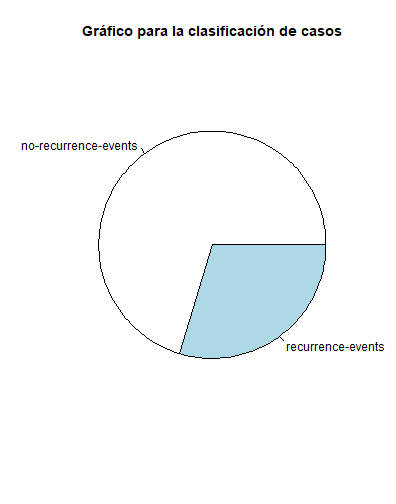
\includegraphics{CapII---P1---Variables-cualitativas_files/figure-latex/unnamed-chunk-10-1} \end{center}

Note que despues de \emph{main} vemos un texto. Este texto es el título
principal (main) del gráfico. Podemos modificar el título, cambiando el
texto dentro de las comillas.

\begin{center}\rule{0.5\linewidth}{0.5pt}\end{center}

Alternativamente, podemos utilizar la librería ggplot para crear un
gráfico de pie con mejor apariencia.

\begin{Shaded}
\begin{Highlighting}[]
\NormalTok{tabla_clase <-}\StringTok{ }\KeywordTok{data.frame}\NormalTok{(}\KeywordTok{table}\NormalTok{(datos}\OperatorTok{$}\NormalTok{clase))}
\KeywordTok{names}\NormalTok{(tabla_clase) <-}\StringTok{ }\KeywordTok{c}\NormalTok{(}\StringTok{"Clase"}\NormalTok{,}\StringTok{"Frecuencia"}\NormalTok{)}

\KeywordTok{library}\NormalTok{(ggplot2)}
\KeywordTok{ggplot}\NormalTok{(tabla_clase, }
       \KeywordTok{aes}\NormalTok{(}\DataTypeTok{x=}\StringTok{""}\NormalTok{, }\DataTypeTok{y=}\NormalTok{Frecuencia, }\DataTypeTok{fill=}\NormalTok{Clase)) }\OperatorTok{+}
\StringTok{  }\KeywordTok{geom_bar}\NormalTok{(}\DataTypeTok{stat=}\StringTok{"identity"}\NormalTok{, }\DataTypeTok{width=}\DecValTok{1}\NormalTok{) }\OperatorTok{+}\StringTok{ }
\StringTok{  }\KeywordTok{coord_polar}\NormalTok{(}\StringTok{"y"}\NormalTok{, }\DataTypeTok{start=}\DecValTok{0}\NormalTok{) }\OperatorTok{+}\StringTok{ }\KeywordTok{theme_void}\NormalTok{()}
\end{Highlighting}
\end{Shaded}

\begin{center}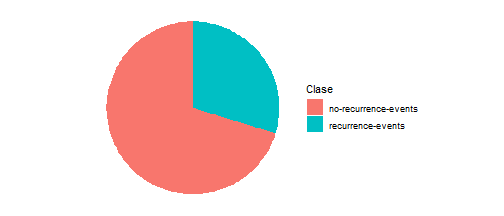
\includegraphics{CapII---P1---Variables-cualitativas_files/figure-latex/unnamed-chunk-11-1} \end{center}

\begin{center}\rule{0.5\linewidth}{0.5pt}\end{center}

\hypertarget{gruxe1fico-de-barras.}{%
\subsection{Gráfico de barras.}\label{gruxe1fico-de-barras.}}

Creamos el gráfico de barras para la variable menopausia.

\begin{Shaded}
\begin{Highlighting}[]
  \KeywordTok{barplot}\NormalTok{(}\KeywordTok{table}\NormalTok{(datos}\OperatorTok{$}\NormalTok{menopausia), }
          \DataTypeTok{xlab=}\StringTok{"Menopausia"}\NormalTok{,}
          \DataTypeTok{ylab=}\StringTok{"Frecuencia"}\NormalTok{,}
          \DataTypeTok{main=}\StringTok{"Distribución de tipos de menopausia"}\NormalTok{)}
\end{Highlighting}
\end{Shaded}

\begin{center}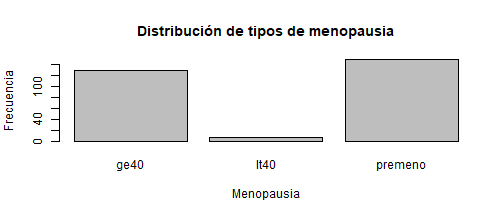
\includegraphics{CapII---P1---Variables-cualitativas_files/figure-latex/unnamed-chunk-12-1} \end{center}

Este gráfico acompaña a la tabla de frecuencias para una visualización
rápida de la distribución de la variable.

name: yourturn template: section

.left-column{[} \# .fancy{[}Ejercicio{]}{]}

\begin{center}\rule{0.5\linewidth}{0.5pt}\end{center}

-name: yourturn1

.right-column{[} Realizar el análisis univariado de las variables del
dataset que no han sido analizadas. Considerar lo siguiente:

\begin{enumerate}
\def\labelenumi{\arabic{enumi}.}
\item
  Explorar la variable .heatinline{[}\textbf{tumor-size}{]} (tamaño del
  tumo) utilizando un gráfico y una tabla de frecuencias. Observar la
  frecuencia y proporciones de cada categoría. Interpretar resultados.
\item
  Explorar la variable .heatinline{[}\textbf{deg-malig}{]} (grado
  histológico del tumor) utilizando un gráfico y tabla de frecuencias.
  Observar la frecuencia y proporciones de cada categoría e interpretar
  resultados.
\item
  Explorar la variable .heatinline{[}\textbf{breast}{]} (lado)
  utilizando un gráfico y tabla de frecuencias. Observar la frecuencia y
  proporciones de cada categoría e interpretar resultados.{]}
\end{enumerate}

.left-column{[} \#\# .fancy{[}.acidinline{[}10:00 minutos{]}{]}{]}

--\textgreater{}

\hypertarget{ejercicios}{%
\section{Ejercicios}\label{ejercicios}}

Realizar el análisis univariado de las variables del dataset que no han
sido analizadas. Considerar lo siguiente:

\begin{enumerate}
\def\labelenumi{\arabic{enumi}.}
\item
  Explorar la variable .heatinline{[}\textbf{tumor-size}{]} (tamaño del
  tumo) utilizando un gráfico y una tabla de frecuencias. Observar la
  frecuencia y proporciones de cada categoría. Interpretar resultados.
\item
  Explorar la variable .heatinline{[}\textbf{deg-malig}{]} (grado
  histológico del tumor) utilizando un gráfico y tabla de frecuencias.
  Observar la frecuencia y proporciones de cada categoría e interpretar
  resultados.
\item
  Explorar la variable .heatinline{[}\textbf{breast}{]} (lado)
  utilizando un gráfico y tabla de frecuencias. Observar la frecuencia y
  proporciones de cada categoría e interpretar resultados.
\end{enumerate}

\hypertarget{otros-materiales}{%
\section{Otros materiales}\label{otros-materiales}}

\begin{itemize}
\tightlist
\item
  \href{https://bookdown.org/jboscomendoza/r-principiantes4/graficas-de-barras.html}{Gráficos
  de barra}
\end{itemize}

setwd(``G:/Mon Drive/6. Trabajos/2021/UNICA/Presentaciones/Grupo
2/Tema2\_Univariado/'')
knitr::purl(``Exploracion\_y\_visualizacion.Rmd'',``1\_Variables\_Cualitativas.R'')

\begin{center}\rule{0.5\linewidth}{0.5pt}\end{center}

---\textgreater{}

\end{document}
